\documentclass[11pt]{article}
\usepackage[a4paper,margin=1in]{geometry}
\usepackage{fourier} % Fourier font
\usepackage{xcolor}
\usepackage{tikz}
\usepackage[most]{tcolorbox}
\usepackage{amsthm, amsmath, amssymb}
\usepackage{enumitem}
\usepackage[hyphens]{url}
\usepackage{hyperref}
\usepackage[nameinlink,noabbrev]{cleveref}
\usepackage{titling} 

% Dark mode colors
\definecolor{bgcolor}{HTML}{FFFFFF}
\definecolor{textcolor}{HTML}{1E1E1E}
\definecolor{defcolor}{HTML}{E86873}
\definecolor{thmcolor}{HTML}{0A9396}
\definecolor{lemcolor}{HTML}{34EB52}
\definecolor{corcolor}{HTML}{9B4AF7}
\definecolor{probcolor}{HTML}{EE9B00}
\definecolor{excolor}{HTML}{0C00F5}

% Background and text color
\pagecolor{bgcolor}
\color{textcolor}

% No paragraph indentation
\setlength{\parindent}{0pt}
\setlength{\parskip}{0.7em}

% Theorem box styles
\tcbset{
  enhanced,
  colback=bgcolor,
  colframe=thmcolor,
  coltext=black,
  coltitle=white,
  fonttitle=\bfseries,
  boxrule=0.7pt,
  left=1em,
  right=1em,
  top=0.7em,
  bottom=0.7em,
  before skip=10pt,
  after skip=10pt,
}

% Theorem environments with colored boxes
\newtcbtheorem[number within=section]{thm}{Theorem}{
  colframe=thmcolor, colback=thmcolor!15!bgcolor
}{thm} % The 'thm' here is the *prefix* for the label

\newtcbtheorem[number within=section]{defn}{Definition}{
  colframe=defcolor, colback=defcolor!15!bgcolor
}{def} % The 'def' here is the *prefix* for the label

\newtcbtheorem[number within=section]{lem}{Lemma}{
  colframe=lemcolor, colback=lemcolor!15!bgcolor
}{lem}

\newtcbtheorem[number within=section]{cor}{Corollary}{
  colframe=corcolor, colback=corcolor!15!bgcolor
}{cor}

\newtcbtheorem[number within=section]{prob}{Problem}{
  colframe=probcolor, colback=probcolor!15!bgcolor
}{prob}

\newtcbtheorem[number within=section]{ex}{Example}{
  colframe=excolor, colback=excolor!15!bgcolor
}{ex}

% Proof environment 
\renewenvironment{proof}[1][\proofname]{%
  \par\pushQED{\qed}\normalfont\topsep6pt \trivlist
  \item[\hskip\labelsep\itshape #1.]\ignorespaces
}{%
  \popQED\endtrivlist\addvspace{6pt}
}

% Cleveref name formats for tcolorbox environments
\crefname{thm}{theorem}{theorems}
\Crefname{thm}{Theorem}{Theorems}

\crefname{def}{definition}{definitions}
\Crefname{def}{Definition}{Definitions}

\crefname{lem}{lemma}{lemmas}
\Crefname{lem}{Lemma}{Lemmas}

\crefname{cor}{corollary}{corollaries}
\Crefname{cor}{Corollary}{Corollaries}

\crefname{prob}{problem}{problems}
\Crefname{prob}{Problem}{Problems}

\crefname{ex}{example}{examples}
\Crefname{ex}{Example}{Examples}

\usepackage{graphicx}



\title{\huge{Semester Project}}
\author{\LARGE{Thobias Høivik} 
    \\ \large{Western Norway University of Applied Sciences} 
\\ \large{ELE201: Microcontrollers and Data Networks}}
\date{}

\begin{document}
\maketitle

\newpage
\tableofcontents

\newpage
\section{Introduction}
In this project we use the STM32 microcontroller along with analog 
sensors 
to gather data that we analyze for statistical and informational 
randomness, 
with the goal of evaluating how feasible such a setup is as a 
hardware-based true random number generator (TRNG). 
The data will be sent via serial connection to a computer 
to analyze the quality of the data.

We will combine theory from information theory, probability, 
signal processing, and networking to assess both the quality of 
randomness 
and how such a system could integrate into a distributed architecture.

We will discuss:
\begin{itemize}
    \item Theoretical background on randomness and entropy.
    \item Implementation and data transfer.
    \item Statistical analysis and randomness testing.
    \item Viability discussion and possible improvements.
    \item Network design for scaling such systems.
\end{itemize}

\newpage
\section{Theory}
\subsection{Randomness and Entropy}
Randomness can be defined both in a statistical and algorithmic sense. 
A sequence is considered random if it is unpredictable and lacks 
compressible structure.

\begin{defn}{Shannon Entropy}{}
Given a discrete random variable $X$ that takes values in $\chi$ with 
probability distribution $p:\chi \to [0,1]$, its entropy is
$$
    H(X) = - \sum_{x \in \chi} p(x) \log_2 p(x).
$$
\end{defn}
(as introduced by Shannon \cite{Shannon1948} 
and discussed in \cite{Gray1990,StatisticShowTo}).
Entropy is a central meassure in information theory pertaining 
to the randomness of data and it will be referenced extensively 
throughout this text.

\subsection{True vs. Pseudo Randomness}
A pseudo-random number generator (PRNG) produces deterministic 
sequences 
from an initial seed, while a true random number generator (TRNG) 
relies 
on physical entropy \cite{HardwareRNGOverview}. 
For hardware-based RNGs, ensuring unbiased and unpredictable output 
requires:
\begin{itemize}
    \item High-quality analog entropy sources.
    \item Statistical post-processing.
\end{itemize}

\subsection{Hypothesis}
We believe that due to the inherit noise of electrical circuits 
that dominate at low frequencies, the 
least significant bits (LSBs) of our signal should be a source of 
high entropy. Then, with further post-processing we should 
get a high-quality source of random numbers which can be applied 
in processes which require randomness.

\newpage
\subsection{Theoretical Modeling of Analog Noise} 
To justify that the least significant bits of our ADC contains 
randomness, we model the analog sensor output as a combination of 
deterministic signal and noise: 
\[ 
    V_{\text{ADC}}(t) = V_{\text{Signal}}(t) + V_{\text{Noise}}(t)
\]

\begin{itemize}
    \item \(V_{\text{Signal}}\) represents the slowly varying, 
        predictable component (e.g. ambient light level in the case 
        of photoresistor). 
    \item \(V_{\text{Noise}}\) represents the unpredictable physical 
        noise (thermal-, shot noise, quantization error, 
        sensor-specific noise).
\end{itemize}

The noise, which is the sum of thermal-, shot-, and other electronic 
noise is typically modeled as a Gaussian random variable 
\cite{Gundersen2019}:
\[ 
    V_{\text{Noise}}(t) \sim \mathcal N(0, \sigma^2_{\text{Noise}}) 
\]

The \textbf{ADC quantization} transforms the continuous voltage 
into discrete levels: 
\begin{align*}
    X = \text{ADC}(V_{\text{ADC}}) \in \{0,1,\dots,2^{12}-1\}
\end{align*}

The voltage corresponding to one LSB (least significant bit) step 
is 
\[ 
    \Delta V = \frac{V_{\text{ref}}}{2^{12}}
\]
for a \(12\)-bit ADC with reference voltage \(V_{\text{ref}}\).


\begin{figure}[h]
    \centering
    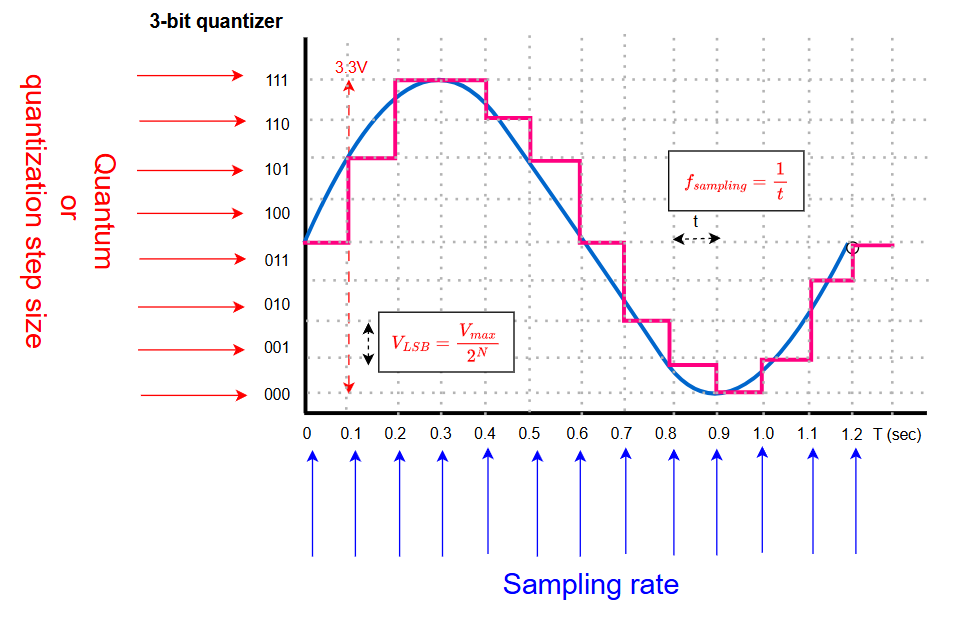
\includegraphics[width=0.8\linewidth]{./images/quantization.png} 
    \caption{Quantization of analog signal.}
    \label{fig:quantization} 
\end{figure}

The randomness of the extracted bits is meassured by the 
Shannon Entropy. For a discrete random variable \(X\) with 
\(k\) possible outcomes, the maximum possible entropy 
\(H_{\text{MAX}} = \log_2(k)\) bits. 

We extract the \(4\) LSBs, which gives \(2^4 = 16\) possible 
outcomes from \(0000_b \to 1111_b\). The maximum entropy then is 
\[ 
    H_{\text{MAX}} = 4 \text{ bits}
\]

Maximum entropy is achieved if the the probability of 
observing any of the \(16\) outcomes is uniform
\cite{Gray1990,StatisticShowTo}:
\[ 
    P(D_{\text{LSB}} = i) = \frac{1}{16} \text{ for } 0 \leq i \leq 15
\]

To achieve a near-uniform distribution across the \(16\) LSB 
states, the standard deviation of the noise \(\sigma_{\text{Noise}}\)
must be large enough to span multiple quantization steps.

Let \(\Delta V_{4-\text{bit}}\) be the voltage corresponding to 
the \(4\) LSBs: 
\[ 
    \Delta V_{4-\text{bit}} = 16\Delta V
\]

Consider an input voltage \(V_{\text{ADC}}\) that falls within 
a \(\Delta V_{4-\text{bit}}\) window. The probability that 
the resulting digital word \(D\) falls into a specific \(4\)-bit 
LSB state \(i\) depends on the area under the Gaussian Probability 
Density function of the noise that falls into the corresponding 
voltage interval \(I_i\). 

The critical condition for near-maximum entropy is then: 
\[ 
    \sigma_{\text{Noise}} \gg \Delta V
\]

If the noise standard deviation is significantly larger than 
the LSB step size then the Gaussian noise distribution becomes 
"smeared" across multiple LSB intervals. Since the noise is 
zero-mean and \(\sigma_{\text{Noise}}\) is large, the probability 
of the total input \(V_{\text{ADC}}\) falling into any one 
LSB interval \(I_i\) is nearly equal to the probability of 
it falling into an adjacent \(I_{i \pm 1}\). 



Just as the least significant bits of the digitized signal capture the high-entropy contributions of analog noise, 
we can also assess the entropy of the signal in the frequency domain. 
By applying the Fourier transform to the analog signal \(x(t)\) and analyzing the normalized power spectral density 
\(p(f_i) = P(f_i) / \sum_j P(f_j)\), we can define the \textit{spectral entropy}
\[
H_{\text{freq}} = - \sum_i p(f_i) \log_2 p(f_i).
\]
A high spectral entropy indicates that the signal’s power is spread across many frequencies, 
consistent with broadband or white noise, while a low entropy suggests structured, 
periodic, or deterministic components \cite{Inouye1991}. 
Thus, the Fourier spectrum provides an alternative viewpoint for identifying regions of high randomness in the signal.

NOTE: REMEMBER TO WRITE PYTHOM PROGRAM TO SHOW THIS

\newpage
\section{Implementation}
\subsection{Hardware Setup}
We will use the STM32f767zi microcontroller, connected to a 
photoresistor.

The microcontroller samples the analog voltage via the ADC and 
stores or 
streams the digital values over a serial or network interface.
We will be sampling at \(12\)-bits, keeping the \(4\) least 
significant bits as we believe these will be most susceptible to 
noise.

NOTE: REMEMBER TO PUT WIRING DIAGRAM HERE.

\subsection{Data Transmission}
Data is transmitted from the STM32 to a computer for analysis. 
In our experimentation we use USART/Serial Connection using 
a micro-usb connection from the microcontroller to a computer.

\newpage
\section{Results and Analysis}
\subsection{Results from the Raw Signal}
We begin by analyzing the apparent randomness 
of the raw signal. 

In our experimentation we first use Python with the serial library 
to read the incoming data and matplotlib to plot the signal 
over time.

\begin{figure}[h]
    \centering
    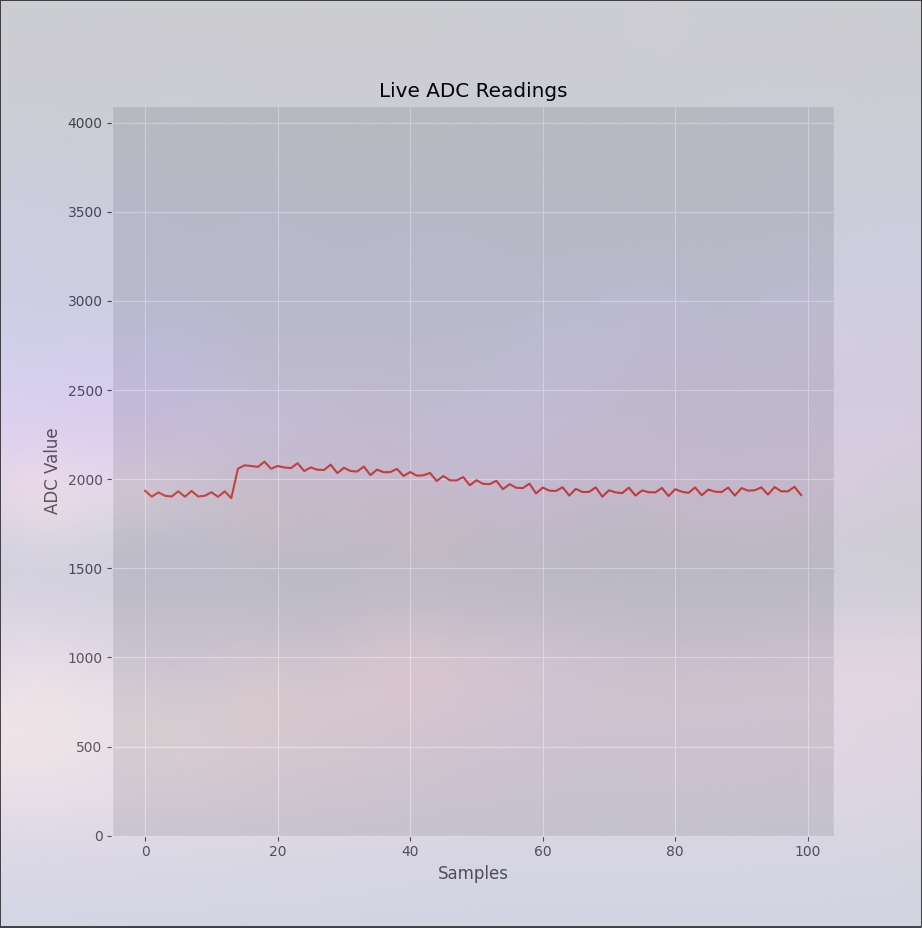
\includegraphics[width=0.6\linewidth]{./images/RAW_READINGS_PLOT.png} 
    \caption{Plot of the raw signal over time}
    \label{fig:raw_signal_plot} 
\end{figure}

As we can see in this plot, while the signal remains relatively stable,
reflecting the stable light level we were testing against, 
there are definite micro-jitters present. This is a good 
sign and is almost ceirtainly due to the noise which we predicted 
would dominate at small levels.

We do have to take into account the fact that the micro-jitters 
might be due to slight fluctuations of the ambient light-level in 
our tests. To mitigate this possibility we will from this time 
forward be testing with the photoresistor covered with electrical 
tape. 

\newpage
Now we look at the observed probabilities pertaining to 
the \(4\) LSBs. We want a roughly equal probability that a given 
bit in the \(4\) LSBs is \(0\) or \(1\).

\begin{figure}[h]
    \centering
    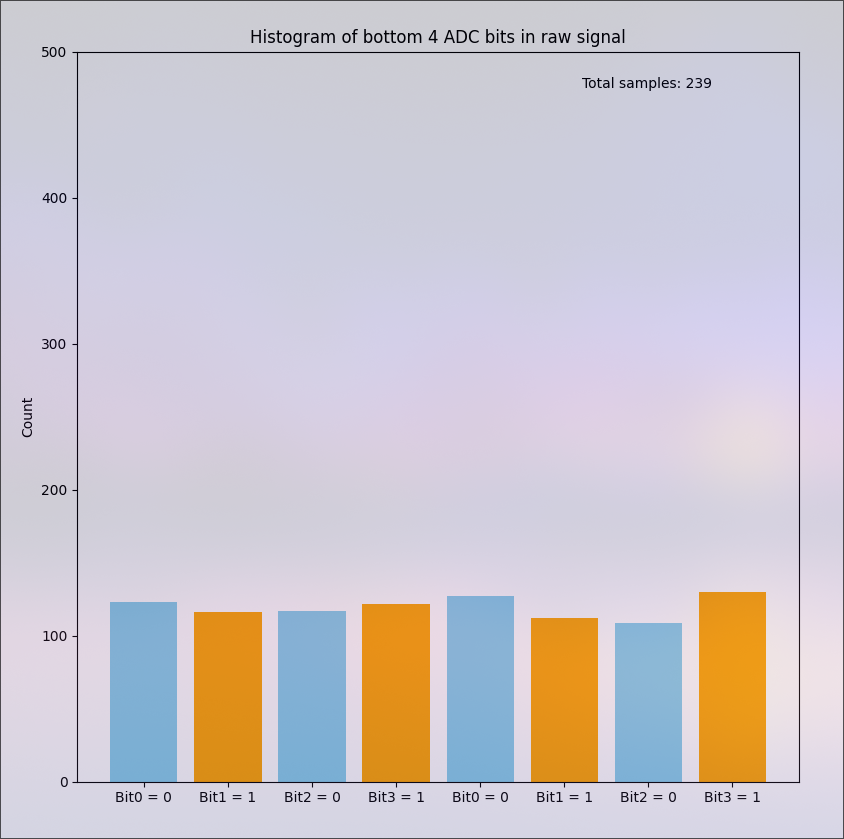
\includegraphics[width=0.6\linewidth]{./images/LSB_HISTOGRAM_COVERED_239.png} 
    \caption{Histogram of 4 LSBs with photoresistor covered}
    \label{fig:histogram_LSB_covered}
\end{figure}

NOTE: Remember to redo this histogram with more samples.

As we can see there appears to be a roughly equal chance that a 
given bit in the \(4\) LSBs is \(0\) or \(1\), pointing towards 
high entropy in the LSBs.
 

\subsection{Processing}
Our goal is to transform the raw data stream 
(which is \textbf{biased} and \textbf{predictable}) into a shorter, 
statistically perfect random stream.

\begin{enumerate}
    \item Raw Bit Extraction 
        \begin{itemize}
            \item \textbf{Technique:} Only use the least significant
                bits of the ADC output. 
            \item The LSBs are dominated by the desired random noise 
                sources and are less influenced by the much larger 
                and more predictable signal 
                (e.g. light level in the case of a light sensor).
                Thus the MSBs should be discarded entirely as they 
                should exibit fairly low entropy.
        \end{itemize}

    \item Entropy Conditioning (Post-Processing) 
        Since the LSBs will more than likely still contain 
        residual bias and correlation we require a powerful 
        \textbf{Entropy Extractor} for cryptographic quality.
        \begin{itemize}
            \item \textbf{XOR Folding:}
                XOR a bit with one a few steps behind. 
                E.g. $\text{Bit}_{\text{Out}} = 
                \text{Bit}_i \oplus \text{Bit}_{i-N}$, 
                where $N$ is chosen to be slightly larger than 
                the observed correlation length.

            \item \textbf{Cryptographic Hash Extractor 
                (NIST SP 800-90B):}
                Collect a large buffer of $L$ raw bits. 
                Estimate $H_{\text{min}}$ per bit. Take the buffer, 
                and hash it (e.g. SHA-256) to produce a fixed-length 
                output.

                Ths downside with this approach is that we have to 
                sample many times to get a sufficiently large buffer.
        \end{itemize}
\end{enumerate}

\subsection{Network Design}
A possible setup:
\begin{itemize}
    \item Each microcontroller is connected to a local router.
    \item A dedicated subnet for sensor nodes (e.g., 192.168.10.0/24).
    \item Central analysis server on a separate subnet.
\end{itemize}

\subsection{Subnetting and Addressing}
We show how to subnet the network efficiently:
\begin{itemize}
    \item Example: dividing a /24 into four /26 subnets.
    \item Assigning IP ranges for sensors, analysis nodes, and administration.
\end{itemize}

\subsection{Data Security and Transmission Integrity}
We briefly discuss:
\begin{itemize}
    \item Packet integrity verification (CRC or checksum).
    \item Optional encryption for data in transit.
    \item Synchronization and time-stamping for accurate sampling.
\end{itemize}

\newpage
\section{Conclusion}
We summarize:Fundamentals of Precision ADC
Noise Analysis
\begin{itemize}
    \item Theoretical feasibility of analog-sensor-based TRNGs.
    \item Experimental results and limitations.
    \item Potential for distributed entropy networks.
\end{itemize}

\subsection{Future Work}
\begin{itemize}
    \item Hardware whitening circuits and amplification.
    \item FPGA or ASIC implementations.
    \item Scaling to larger networks and entropy pooling.
\end{itemize}

\newpage
\begin{thebibliography}{99}  
    \raggedright

\bibitem{Shannon1948}
C. E. Shannon,
\textit{A Mathematical Theory of Communication},
Bell System Technical Journal,
vol. 27, pp. 379--423, 623--656, 1948.

\bibitem{Gray1990}
R. M. Gray,
\textit{Entropy and Information Theory},
Springer, 1990.

\bibitem{HardwareRNGOverview}
Cerberus Security,
\textit{Hardware Random Number Generators},
2020.
\url{https://cerberus-laboratories.com/blog/random_number_generators/}

\bibitem{StatisticShowTo}
Statistics How To,
\textit{Shannon Entropy Definition},
\url{https://www.statisticshowto.com/shannon-entropy/}

\bibitem{Gundersen2019}
G. Gundersen,
\textit{Random Noise and the Central Limit Theorem},
Blog post, 01 February 2019.
\url{https://gregorygundersen.com/blog/2019/02/01/clt/}


\bibitem{Inouye1991}
T. Inouye, K. Shinosaki, et al.,
\textit{Quantification of EEG irregularity by use of the entropy of the power spectrum},
Electroencephalography and Clinical Neurophysiology, 79(3):204–210, 1991.
\url{https://doi.org/10.1016/0013-4694(91)90138-6}

\end{thebibliography}

\end{document}

